% Preamble
\documentclass[../main.tex]{subfiles}

% Document
\begin{document}
\chapter{Python code implementation}\label{ch:annex}

This appendix presents the Python code used for the implementation of the simulator, 
the $\epsilon$-Greedy, UCB, TS, LinUCB, and LinTS algorithms, and the training of 
these models using the data generated by the simulator. All this code is available 
in the GitHub repository accessible at the following URL: 
\url{https://github.com/Eduard0LP/MABE-Multi-Armed-Bandits-for-E-commerce}.  

The implementation of all code related to the models and the simulator was carried out 
using only the NumPy and Pandas libraries as dependencies. In addition to these libraries, 
scikit-learn was also used for encoding categorical variables into numerical variables 
during the training of the linear regressions of the contextual algorithms, and 
Matplotlib and Seaborn were used for the graphical representation of the results.  

Regarding the simulator, the function that generates the users who will be the potential 
customers of the e-commerce platform was called \textit{generate\_user} and returns the 
data of a user in a Python dictionary. Its implementation can be seen in Figure 
\ref{fig:generate_user_function}.  

\begin{figure}[H]
\centering
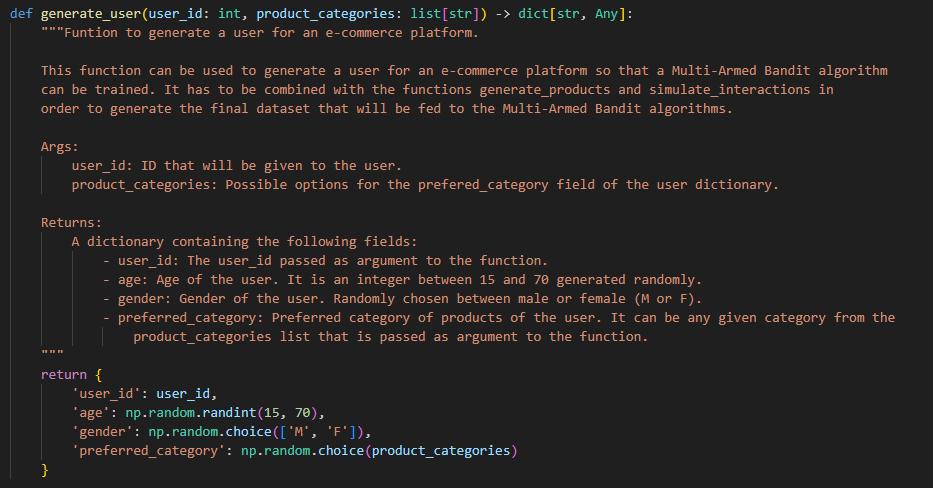
\includegraphics[width=140mm]{../img/generate_user_function.png}
\caption{Python function used to generate the website users.}
\label{fig:generate_user_function}
\end{figure}

The products were generated using the  \textit{generate\_products} function (Figure 
\ref{fig:generate_products_function}), which returns a Pandas DataFrame containing the 
data of all available products.  

\begin{figure}[H]
\centering
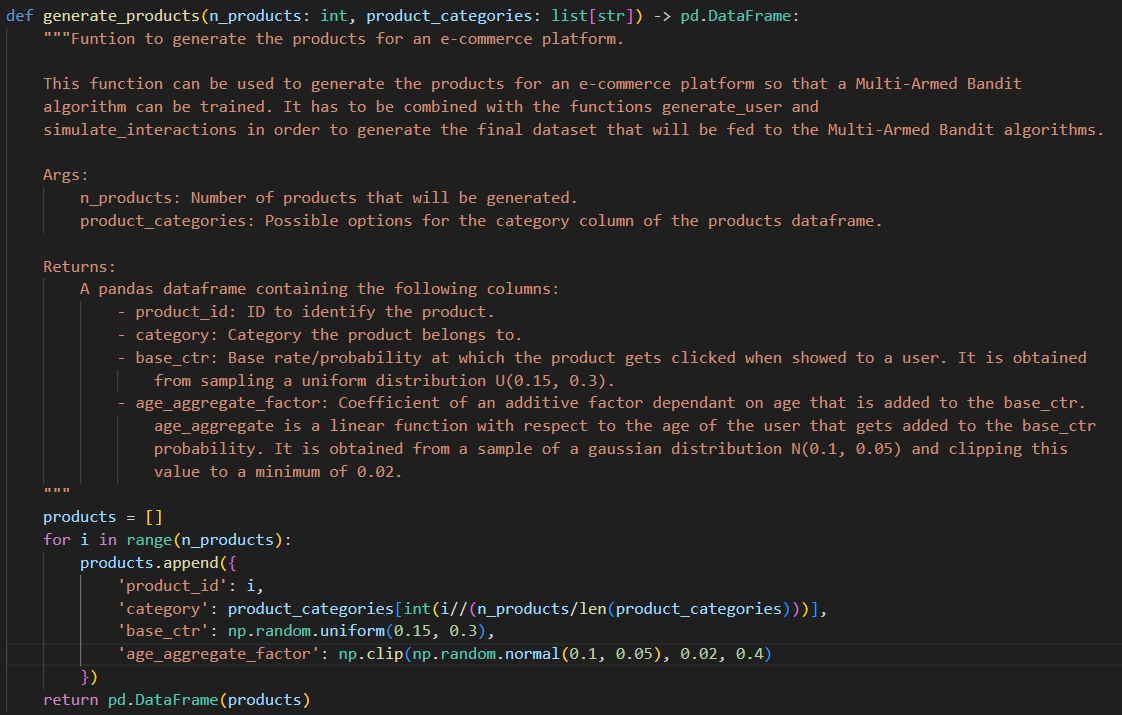
\includegraphics[width=140mm]{../img/generate_products_function.png}
\caption{Python function used to generate the website products.}
\label{fig:generate_products_function}
\end{figure}

\begin{figure}[H]
\centering
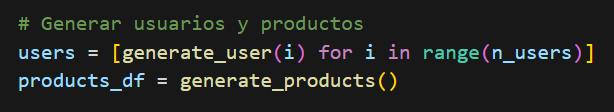
\includegraphics[width=140mm]{../img/generate_user_and_product_call.png}
\caption{Code snippet in which the \textit{generate\_user} and \textit{generate\_products} 
functions are called to generate the users and the products.}
\label{fig:generate_user_and_product_call}
\end{figure}

The third and final component of the simulator, as mentioned in the methodology section, 
was responsible for simulating the interactions between users and products. This was 
implemented with the \textit{simulate\_interactions} function, which receives the user 
data generated by \textit{generate\_user} and the DataFrame generated by 
\textit{generate\_products}, and simulates whether that user would click or not on each 
product in the DataFrame if it were recommended to them. The results of all these simulations 
are returned in a new DataFrame. The implementation of this function can be seen in Figure 
\ref{fig:simulate_interactions_functions}.  

\begin{figure}[H]
\centering
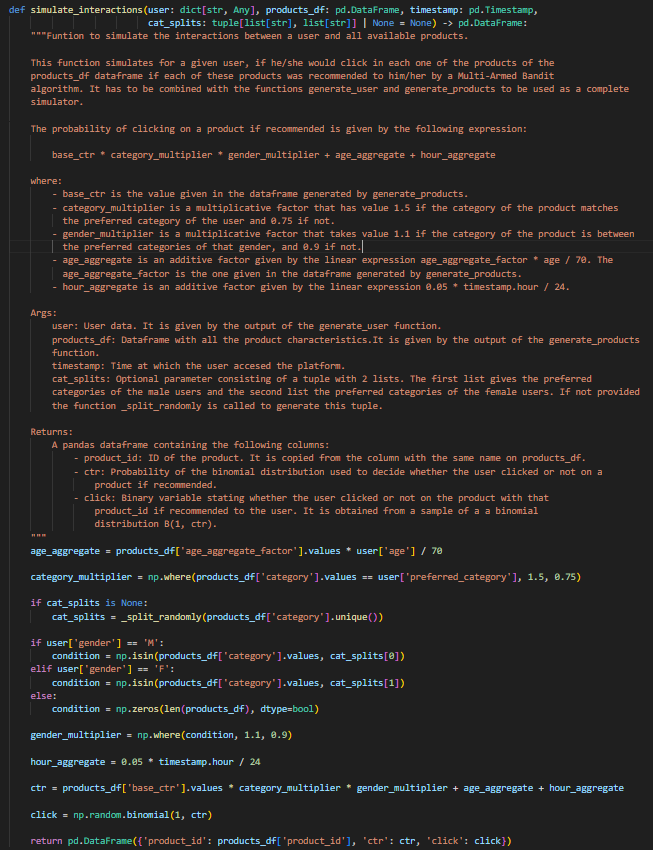
\includegraphics[width=140mm]{../img/simulate_interactions_functions.png}
\caption{Python function to simulate product–customer interactions.}
\label{fig:simulate_interactions_functions}
\end{figure}

Regarding the implementations of the algorithms discussed in this work, these were implemented 
using Python classes with three main methods: an \textit{\_\_init\_\_} method to initialize the 
class with the appropriate parameterization of the algorithm, a \textit{select\_action} method 
through which the algorithm makes the recommendation of a product based on the context, and an 
\textit{update} method to update the algorithm’s parameters after receiving the result of whether 
the recommendation received a reward or not. It is important to emphasize that even for algorithms 
that do not use context, it is still passed to the \textit{select\_action} and \textit{update} 
methods, and it is simply ignored within those classes.  

This design choice was made to maintain exactly the same interface across all models, thus 
facilitating the simultaneous training of all of them within a single training loop using the 
simulator. The implementations of all these models can be seen in Figures 
\ref{fig:epsilon_greedy_model}, \ref{fig:ucb_model}, \ref{fig:ts_model}, \ref{fig:linucb_model}, 
and \ref{fig:lints_model}. Regarding the training of all models, it was carried out jointly in 
the training loop shown in Figure \ref{fig:simultaneous_train}.  

\begin{figure}[H]
\centering
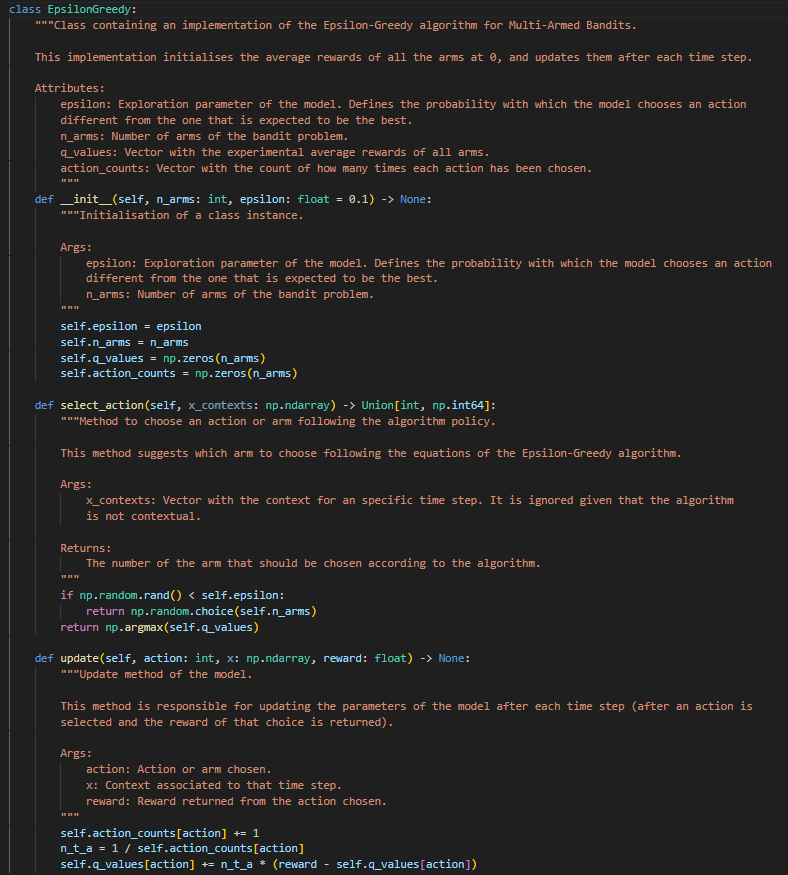
\includegraphics[width=140mm]{../img/epsilon_greedy_model.png}
\caption{Python class implementing the $\epsilon$-Greedy algorithm.}
\label{fig:epsilon_greedy_model}
\end{figure}

\begin{figure}[H]
\centering
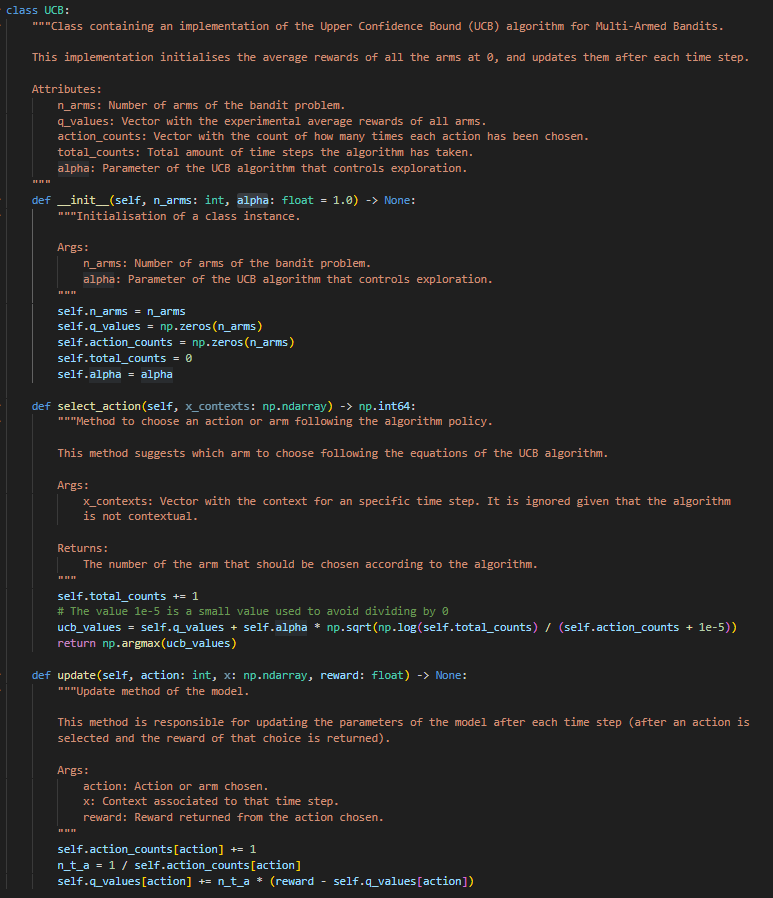
\includegraphics[width=140mm]{../img/ucb_model.png}
\caption{Python class implementing the Upper Confidence Bound algorithm.}
\label{fig:ucb_model}
\end{figure}

\begin{figure}[H]
\centering
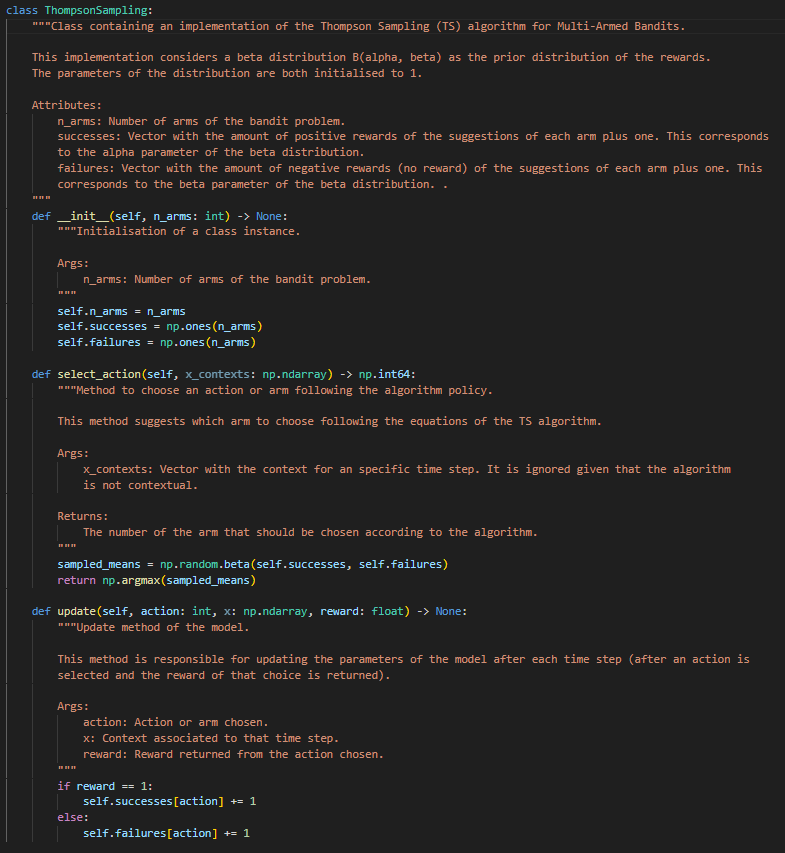
\includegraphics[width=140mm]{../img/ts_model.png}
\caption{Python class implementing the Thompson Sampling algorithm.}
\label{fig:ts_model}
\end{figure}

\begin{figure}[H]
\centering
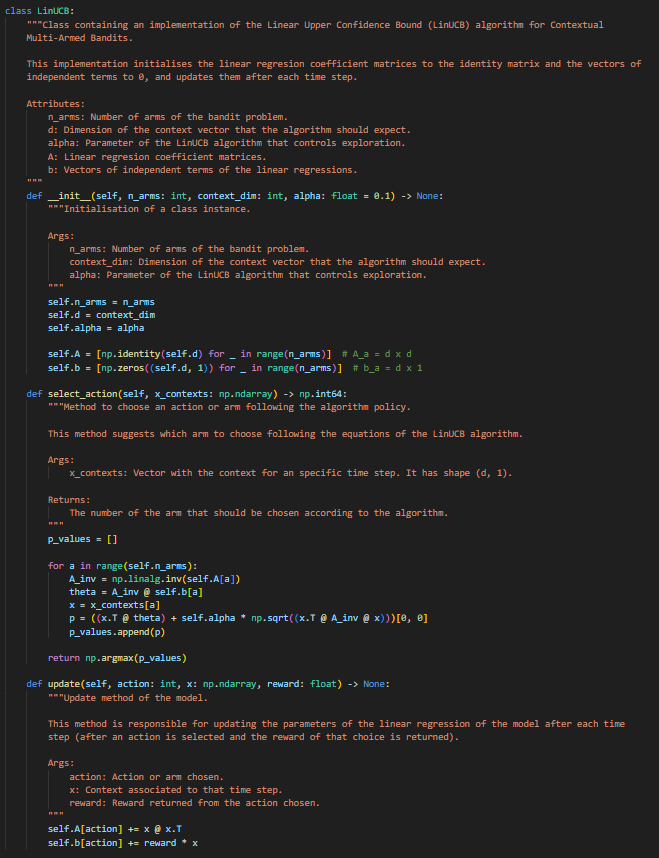
\includegraphics[width=140mm]{../img/linucb_model.png}
\caption{Python class implementing the Linear Upper Confidence Bound algorithm.}
\label{fig:linucb_model}
\end{figure}


\begin{figure}[H]
\centering
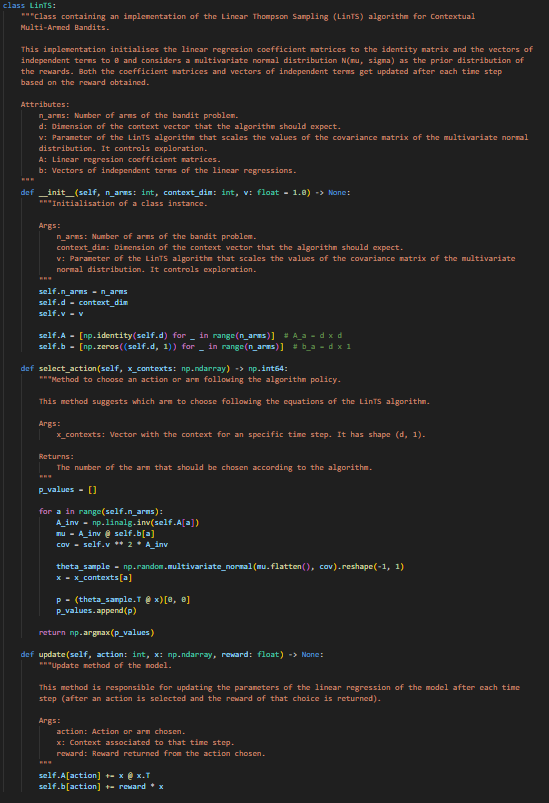
\includegraphics[width=140mm]{../img/lints_model.png}
\caption{Python class implementing the Linear Thompson Sampling algorithm.}
\label{fig:lints_model}
\end{figure}

\begin{figure}[H]
\centering
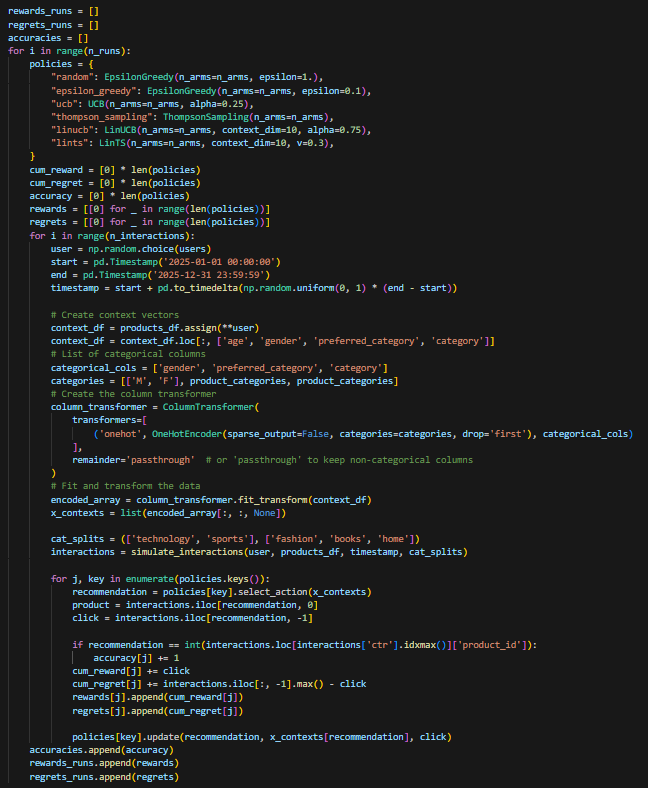
\includegraphics[width=140mm]{../img/simultaneous_train.png}
\caption{Simultaneous training of all algorithms.}
\label{fig:simultaneous_train}
\end{figure}

\end{document}